Language models are known to contain knowledge on their own \citep{petroni2019language,petroni2020how} and we cover the extraction of this knowledge in a later chapter.
Consider a question answering system based on a large language model.
When asked about the current president, it is able to provide the correct answer.
But on the day of inauguration, the true answer will be different while the model will keep the old one.
Because the information about the current president is stored in the model's parameters, the only reliable way of updating this information in the model is to fine-tune it or re-train it from scratch.
However, changing a small piece of information should not require these complicated and expensive operations.
For this, we turn to knowledge-enhanced language models.

Models which contain information indirectly in their parameters are called \defn{parametric} \index{parametric} \index{non-parametric} and their counterparts, models which rely on external information, are called \defn{non-parametric}.
They do have parameters but most of the information is not stored there but in some other form and location, called a \textit{knowledge base}.
This can be in human-accessible form, such as the heap of Wikipedia articles, but also in a more structured format, such as a knowledge graph.

The general principle is that during the inference, the model generates a key by which an external, interpretable, and editable system is queried.
Next, the result of this search is fused into the model and the inference continues.
Continuing with the question answering example, the model may construct e.g. an SQL query for the current president in a given country.
Upon receiving the answer, it is attended to in the inference and used in producing the output.
When the true answer changes e.g. on the inauguration day, it can easily be edited by a human or another automated system in the database and the large language model, which serves as question answerer, does not need to be changed at all.
To summarize, the advantage of having an external source of information is:
\begin{itemize}
    \item models cannot memorize all knowledge in their parameters, especially long-tail knowledge,
    \item model's knowledge can be easily updated with the latest information without expensive training,
    \item output is interpretable and verifiable because we can later examine which pieces of information were retrieved and used in the inference process,
    \item non-parametric models with fewer parameters can achieve better results than parametric larger models.
\end{itemize}


\paragraph{Hallucination}
LLMs are capable of generating coherent text, however, the generated text is not always factually correct as in the question answering example from the previous paragraph. This is commonly referred to as a hallucination. Retrieval augmentation is one of the approaches to mitigate hallucination. 

The goal is to reduce the hallucination of a model, but first we should have a measure or metric. However, it is challenging to measure hallucinations and there is no single metric covering all aspects and tasks. Many traditional generation metrics use human-annotated ground-truth references (such as BLEU \citep{papineni2002bleu}, ROUGE \citep{lin2004rouge}, …). However, there are many possible generations for the same input text, and collecting all possible outputs is impossible. Therefore, some hallucination metrics rely just on the source text as a sole reference. For example, the Knowledge-F1 \citep{shuster-etal-2021-retrieval-augmentation} metric used in knowledge-grounded dialogues measures the overlap between the model generation and knowledge used to ground the dialogue.
Other approaches use models to measure the hallucination degree given a source and generated text. These metrics handle more complex semantic variations of generation. However, these metrics are prone to errors for out-of-training data texts. 
One example of such metrics is $Q^2$ \citep{honovich-etal-2021-q2}, which first generates question-answer pairs given a generated text, and then uses a QA model to answer the generated questions given a source text. The final score is measured as a similarity between answers using an NLI model.


\begin{figure}[h]
    \centering
    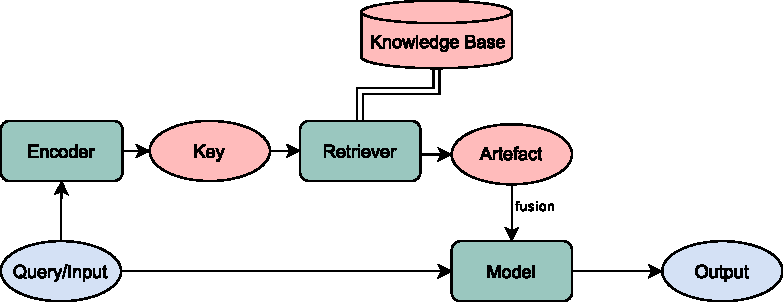
\includegraphics[width=0.8\textwidth]{figures/multimodality/artefacts_diagram.pdf}
    \caption{Retrieval augmented generation (RAG) scheme. Artefacts are retrieved from a knowledge base by Retriever and fused them into the Model to produce a better output. Adapted from \citet{zouhar2021artefact}.}
    \label{fig:rag-idea}
\end{figure}

\section{Prototypical RAG}
The simplest way to approach knowledge enhancement of LLM is to retrieve relevant documents from external knowledge sources and add them as input to the model during inference. This approach is an example of a non-parametric model which can rely on external information rather than remember the facts in weights. The general scheme of such a system is shown in Figure \ref{fig:rag-idea} with the fusion of retrieved knowledge as a simple concatenation.
Prototypical approach to RAG involves two main stages: 
\begin{itemize}[noitemsep]
    \item retrieval of relevant documents to a user query and,
    \item generation which given relevant documents either extracts the answer or generates the answer, 
\end{itemize}
and each component is trained independently.

The goal of the retrieval is to find a small subset of elements that are most similar to the query $q$ 
\begin{align}
    \textsc{ArgTop-k}\, \textsc{sim}_{d \in \mathcal{D}}(q,d), 
\end{align}
where $\textsc{sim}$ is the similarity score between two pieces of text.
Existing retrieval methods can be categorized based on a vector dimensionality into sparse retrieval and dense retrieval approaches.

\paragraph{Sparse Retrieval} The most widely used methods of sparse retrieval are TF-IDF \citep{robertson1997relevance} and BM25 \citep{robertson2009probabilistic}.
TF-IDF (term frequency-inverse document frequency) is a measure of the importance of a term in a document based on how often the term appears in a given collection of documents. If a term appears frequently in a document, it is important and we should get a high score. However, if the term appear in majority of documents, it is probably a common word and the score should be lower. The formula is:

\begin{align} 
\text{tf-idf}(t, d, \mathcal{D}) = \text{tf}(t, d) \times \text{idf}(t, \mathcal{D}) \\ \text{tf}(t, d) = \log(1 + \text{freq}(t, d)) \\ \text{idf}(t, \mathcal{D}) = \log \Big( \frac{\vert\mathcal{D}\vert}{\vert d \in \mathcal{D}: t\in d\vert} \Big) 
\end{align}
where $t$ is term, $d$ is a document from a collection of documents $\mathcal{D}$, and $\text{freq}(t, d)$ measures how many times a term $t$ appears in document $d$. 
The disadvantage of these methods is that the dimension of vectors is the same as the number of terms in a vocabulary and term matching is limited for several scenarios such as when synonyms are used. 

\paragraph{Dense Retrieval}
The modern approaches to the retrieval are using dense retrieval which overcomes the limitations of sparse models that require high term overlap between a query and a document.  An example of such an approach is the Dense Passage Retrieval model (DPR) \citep{karpukhin2020dense}. The model follows a dual encoder scheme to map questions $q$ and documents $d$ into $h$--dimensional vector and use dot product as a similarity measure:
\begin{align}
   \textsc{sim}(q, d) = \textsc{encoder}(q)^T \cdot \textsc{encoder}(d). 
\end{align}
The goal of the encoders training is to use contrastive learning to learn an embedding function to create a vector space such that relevant pairs of questions and documents are closer to each other (high similarity, low distance) than the irrelevant ones. Let $\mathcal{D}=\{q_i, d_i^+, d_{i,1}^-, ..., d_{i,n}^-\}_{i=1}^m$ be the training data with one positive document and $n$ irrelevant documents (such as random, hard negatives from BM25, ...). The loss function optimizes the negative log-likelihood of the positive document:
\begin{align}
    L(q_i, d_i^+, d_{i,1}^-, ..., d_{i,n}^-) = -\log \frac{e^{\textsc{sim}(q_i,d_i^+)}}{e^{\textsc{sim}(q_i,d_i^+)}+\sum_{j=1}^{n}e^{\textsc{sim}(q_i,d_{i,j}^-)}}
\end{align}

The encoder used in their work is a pre-trained BERT model and they take the representation at the \textit{[CLS]} token as the output, so $h=768$. The performance of the DPR model outperforms sparse methods such as BM25 as shown in \Cref{fig:dpr-results}.

\begin{figure}
    \centering
    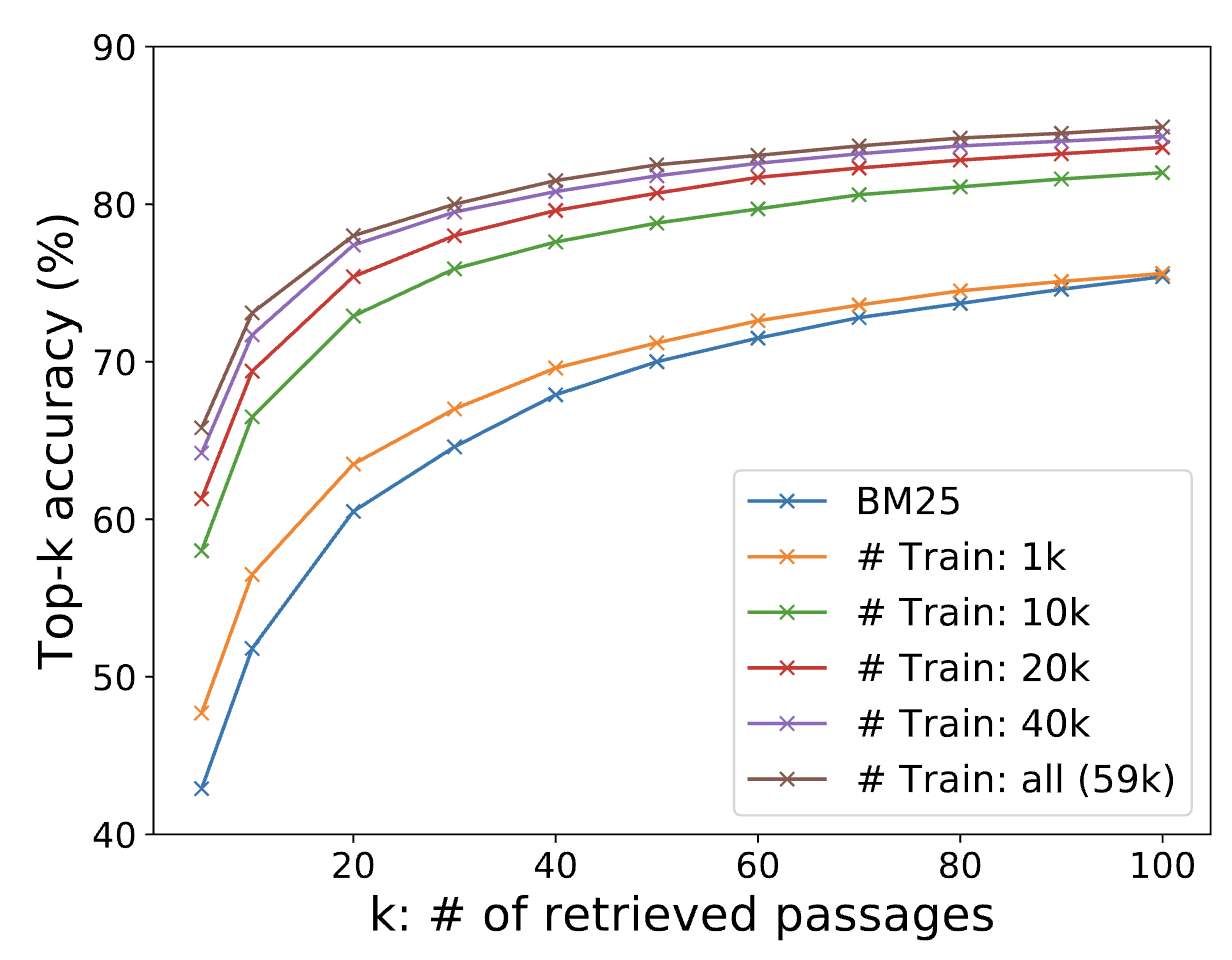
\includegraphics[width=0.5\textwidth]{figures/multimodality/dpr-results.png}
    \caption{Retrieved top-k accuracy with a different number of training examples. DPR outperforms the sparse retrieval approach BM25 with only 1000 training samples. Taken from \citep{karpukhin2020dense} }
    \label{fig:dpr-results}
\end{figure}


\paragraph{Retrieval Metrics}
Common metrics for evaluating the retrieval part are those that consider the ranking order of results, such as \defn{Recall at $k$} \index{Recall at $k$} (R@k) and \defn{Mean Reciprocal Rank} \index{Mean Reciprocal Rank} (MRR).
Both metrics are averaged across multiple queries, e.g. a whole dataset.
\begin{align}
\textsc{R}@k &= \frac{|\text{retrieved documents}\cap \text{relevant documents} |}{|\text{relevant documents} |} \\
\textsc{MRR} &= \frac{1}{\text{rank of first relevant document}}
\end{align}

\paragraph{Model example}
An example of a prototypical RAG system is DrQA (Document retriever Question-Answering) \citep{chen-etal-2017-reading}, which uses a fixed TF-IDF for retrieval and a reading comprehension model to extract the answer from retrieved documents. With the rise of generative models, Fusion-in-decoder models \citep{izacard-grave-2021-leveraging} show prompting models to generate answers from relevant documents instead of extracting them leads to better results.  However, independent training limits retrieval models not being optimized for the task or the domain, and the second stage (reader or generation) is not trained to leverage retrieval. 


\section{Models}
We now describe more in detail several models that use the knowledge retrieval approach.
An important distinction between these models is how they use the retrieved artefact.
A generative model or pipeline, given input $x$, can be thought of as a composition of some functions: $f_1(f_2(f_3(f_4(x))))$.
Then, with the retrieved artefact $a$ (e.g. document), we can add it for example at the beginning of the inference: $f_1(f_2(f_3(f_4(x, a))))$, in the middle, or at the very end: $f_1(f_2(f_3(f_4(x))), a)$.
This is referred to as \defn{fusion} \index{fusion} (\Cref{fig:rag-idea}) with the first one being early fusion and the second being late fusion.
The particular mechanics of fusion covered in the following subsections are:
% , as demonstrated by the following models, range from simple text concatentation to more sophisticated aggregation.
\begin{itemize}
    \item Fuse artefact in the input layer by concatenation - REALM,
    \item Fuse artefact in the intermediate layers by cross attention - RETRO,
    \item Fuse artefact in the output layer by interpolating LM output probability - kNN LM.
\end{itemize}

\subsection{REALM}

\begin{figure}[h]
    \centering
    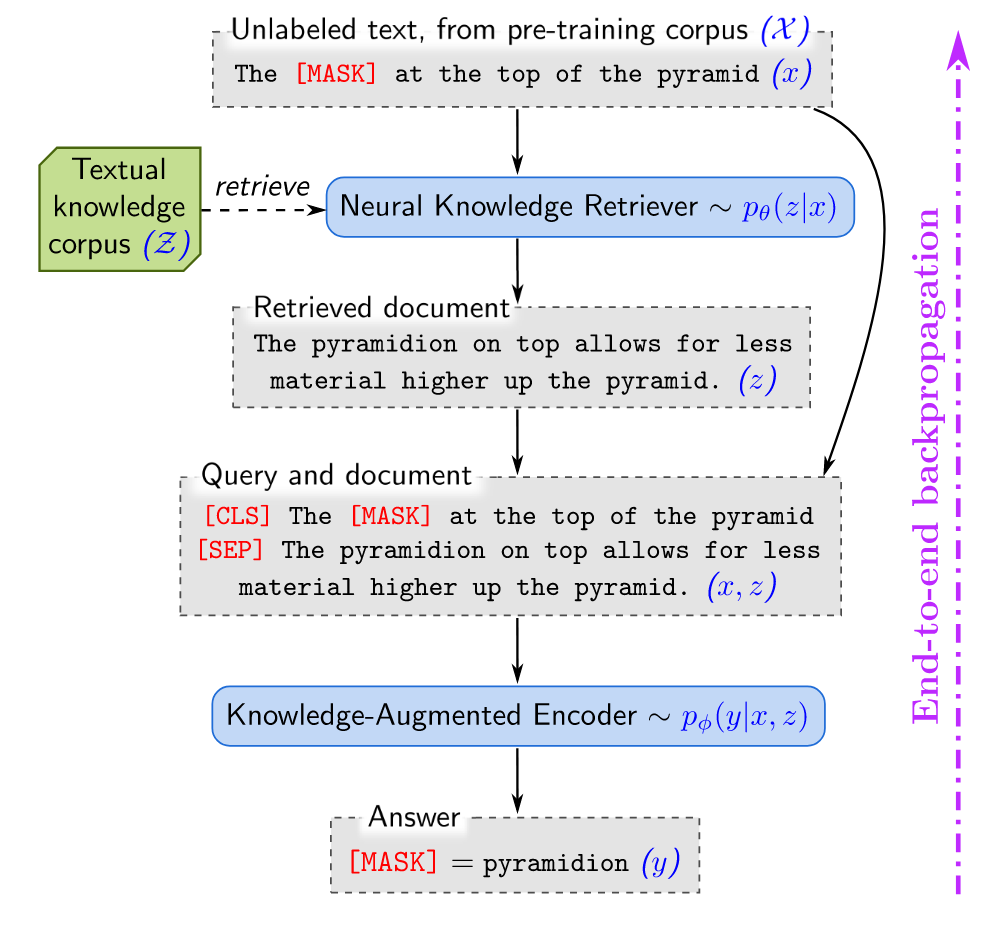
\includegraphics[width=0.5\textwidth]{figures/multimodality/realm.png}
    \caption{REALM augments LM MLM pre-training with a retriever (Neural Knowledge Retriever) which retrieves knowledge from a corpus of documents $Z$ (e.g. Wikipedia). Backpropagation is done through both components. Because the retriever must consider millions of documents in $Z$, REALM approximates this by using top $k$ documents. }
    \label{fig:realm}
\end{figure}

\begin{figure}[h!]
    \centering
    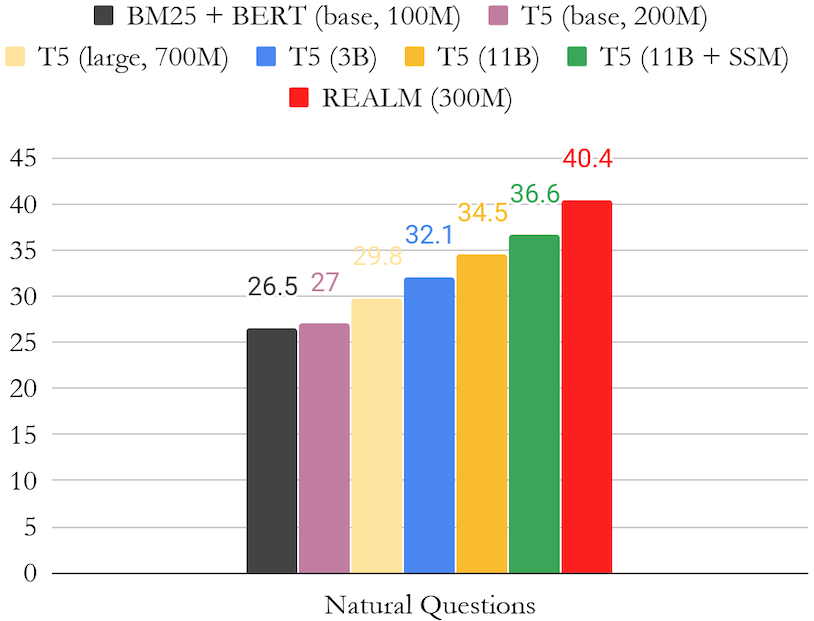
\includegraphics[width=0.5\textwidth]{figures/multimodality/realm-results.png}
    \caption{Open-domain QA accuracies of various models on the Natural Question dataset. REALM outperforms sparse-retrieval approaches (BM25 + BERT) and no retrieval baselines (T5 versions). SSLM refers to salient span masking. Taken from Google Research Blog.}
    \label{fig:realm-results}
\end{figure}

REALM \citep{guu2020retrieval} decomposes $p(y|x)$ into \textit{retrieve} and \textit{predict} steps and optimize them jointly as shown in \Cref{fig:realm}. Given an input $x$, the model first retrieve useful documents $z$ from corpus $Z$ by sampling from the distribution $p(z|x)$. In the predict step, the model condition both on input $x$ and retrieved $z$ which is modeled as $p(y|z,x)$. To obtain the likelihood of generating $y$, REALM treats $z$ as a latent variable and marginalizes over all possible documents $z$
\begin{align}
& \texttt{Model output:} & \hspace{2.6cm} p(y|x)= \sum{p(y|z,x) p(z|x)}
\end{align}
The retriever is based on DPR \citep{karpukhin2020dense} and is defined as a bi-encoder architecture:
\begin{align}
& \texttt{Retriever:} & \hspace{0.6cm} p(z|x) = \exp(\textsc{encoder}(z)^T \cdot \textsc{encoder}(x)),
\end{align}
which means relevance between document $z$ and input $x$ is defined as the inner product of their encoder representations. 
The predict step simply concatenate $z$ and $x$ into one sequence and jointly trains the model first using MLM followed by fine-tuning on the open-domain QA task. \citep{lewis2020retrieval} extend this work with a generative model (BART) instead of MLM, fine-tuned on open-domain QA and knowledge-intensive tasks. 

To summarize, REALM and \citep{lewis2020retrieval} retrieve text passages, fuse them by concatenating them to the input, and in contrast to prototypical RAG, jointly optimize both components. \Cref{fig:realm-results} shows REALM outperforms both sparse retrieval baselines and parametric models.




\subsection{RETRO}
The idea of the RETRO (Retrieval Enhanced TRansfOrmers) model \citep{borgeaud2022improving} is to incorporate artefact into the intermediate layer instead of the input layer. RETRO is a fully autoregressive model and uses text chunks which are larger than one token due to scalability. 
As shown in the \Cref{fig:retro-arch}, the model uses encoder-decoder transformer architecture and fuse artefact into model using chunked cross-attention mechanism (CCA) \citep{vaswani2017attention}.

\begin{figure}[h]
    \centering
    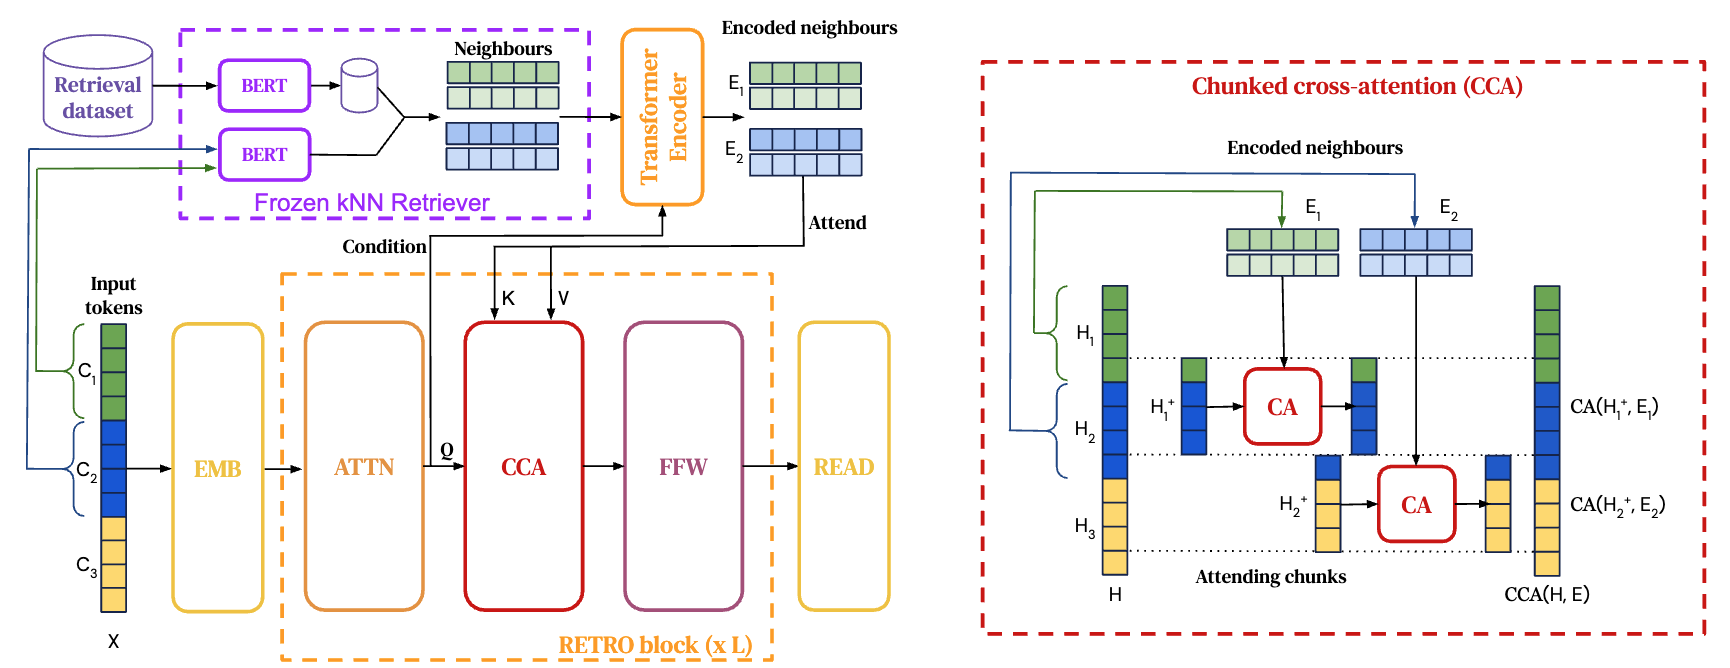
\includegraphics[width=0.8\textwidth]{figures/multimodality/retro-arch.png}
    \caption{Left: Example of the RETRO architecture with 3 text chunks $C$ of 4 tokens in size, with 2 retrieved neigbours with 5 tokens each. Neigbours are encoded and the decoder uses RETRO blocks with self-attention and cross-attention. Right: Detail of the chunked cross-attention. Taken from \citet{borgeaud2022improving}.}
    \label{fig:retro-arch}
\end{figure}

The retriever is based on DPR \citep{karpukhin2020dense} and is defined as a bi-encoder architecture using a frozen BERT model:
\begin{align}
& \texttt{Retriever:} & \hspace{0.6cm}\exp(\textsc{encoder}(z)^T \cdot \textsc{encoder}(x)),
\end{align}
First, for each text chunk $C$, top-k nearest neighbours $RET(C_u)$ are filtered using L2 distance on BERT embeddings.

The retrieved neigbours chunks are fed into a bi-directional transformer encoder:
\begin{align}
& \texttt{Encoder:} & E_u^j = \textsc{encoder}(\textsc{RET}(C_u)^j, H_u)),
\end{align}
where $j\in[1, k]$ is an index of neighbour and $H_u$ are intermediate activations of chunk $C_u$.
Compared to regular decoder Transformer blocks, RETRO interleaves standard transformer blocks $\textsc{LM}(H)$ with self-attention $\textsc{ATTN}(H)$, and RETRO-blocks $\textsc{RETRO}(H, E)$ with chunked cross-attention $\textsc{CCA}(\textsc{ATTN}(H), E)$. 

To summarize, the RETRO model fuses artefact into an intermediate layer using cross-attention. This results in both more accurate and more factual continuations, and it has been shown the model outperform parametric models which are 25x bigger.


\subsection{kNN LM}
Concatenation to the input or intermediate layers is not the only possible approach to the retrieval. In KNN LM proposed by \citet{khandelwal2019generalization}, the model retrieves nearest neighbours tokens and uses them at the output layer level.
The language model utilizes memorization of the training data during inference to predict otherwise sparsely occurring words.
In this approach, the authors first compute representations of all sentence prefixes (last self-attention layer) and store them as a mapping to the following word:
% The representations ($1024$ dimensions) are the output of the last self-attention layer of the trained Transformer-based language model.
\begin{align}
& \texttt{Encoder:} & k = \textsc{LM}^\text{rep.}(X_{<i}) \\
& \texttt{Datastore}: & \mathcal{B} = \{ (\texttt{Encoder}(X_{<i}), X_{i}) |X\in D_\text{train}, i < |X| \}
\end{align}
In autoregressive inference, the prefix is again computed for the current sentence and then $1024$ neighbours in the vector space are retrieved:
\begin{align}
& \texttt{Retriever:} & \hspace{2.6cm} S = \{(r, v) |(r, v) \in \mathcal{N}_{1024}^{L^2}(k)\}
\end{align}
Then, their corresponding mapped words are combined together into a single distribution over the vocabulary:
\begin{align}
& \texttt{Aggregator:} & \hspace{1cm} p_\xi(\hat{X}_i) \propto \sum_{(r,v) \in S} \mathbbm{1}_{v} \exp(-||r-k||_2 \cdot v)
\end{align}
Formally, this alone would create its own kNN-based language model $p_\xi$.
However, its output is weighted to the main model's own prediction using manually set hyperparameter $\lambda \in [0,1]$.
The higher it is, the more weight is put to the retrieved prediction as opposed to the current model's prediction:
\begin{align}
& \texttt{Model output:} & \hspace{2.5cm} \lambda \cdot p_\xi + (1-\lambda) \cdot \textsc{LM}(X_{<i}) \label{eq:knn_lm_final}
\end{align}

% They then use this for the next word prediction by softmaxing negative $L^2$ distances\footnote{The negative $L^2$ distance is used instead of the common inner product as the similarity measure. This was shown empirically by the authors to work better.} of $1024$ neighbours.
The symbolic working of the model is shown in the following set of equations and \Cref{fig:knn_lm} which is adapted from the original paper.
% The importance of the retrieved words in the output is determined by the manually set hyperparameter $\lambda \in [0,1]$, resulting in linear (convex) interpolation.
% The aggregator is the softmax function; $\text{LM}^\text{rep.}(X_{<i})$ is the vector representation of the prefix $X_{<i}$ by the trained language model.
Even with preserving the same amount of trainable parameters, the perplexity on WikiText-103 of a baseline model \citep{baevski2018adaptive} was reduced from $18.7$ to $15.8$.

\begin{figure}[htbp]
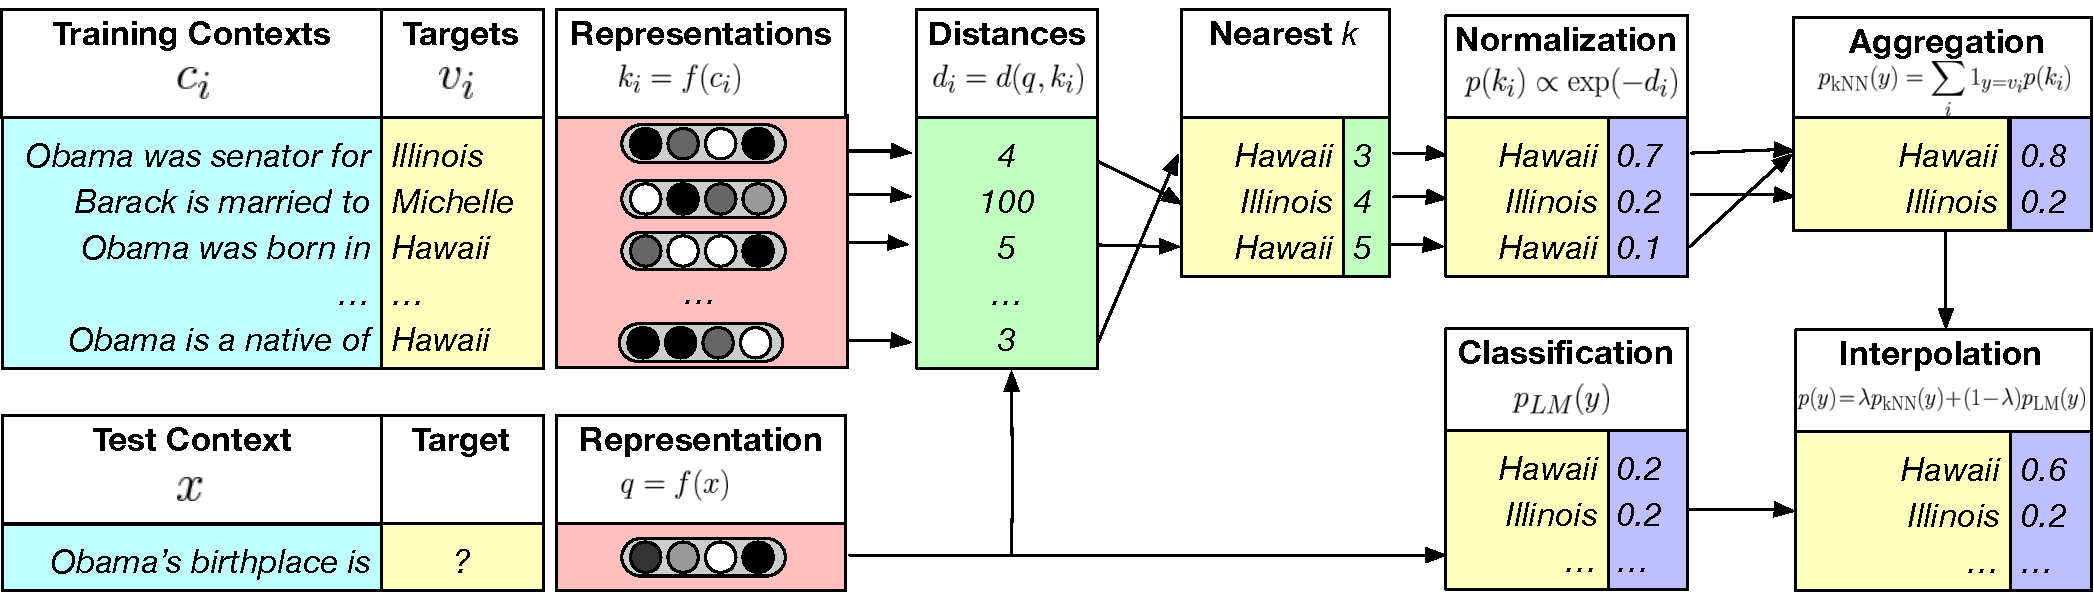
\includegraphics[width=\linewidth]{figures/multimodality/knn_lm_diagram.pdf}
\caption{An illustration of kNN-LM. A datastore is constructed with an entry for each training set token, and an encoding of its leftward context. For inference, a test context is encoded, and the $k$ most similar training contexts are retrieved from the datastore, along with the corresponding targets.
A distribution over targets is computed based on the distance of the corresponding context from the test context.
This distribution is then interpolated with the original model’s output distribution. \citep{khandelwal2019generalization}}
\label{fig:knn_lm}
\end{figure}

To summarize, kNN LM retrieves tokens at every token prediction step. This is a more fine-grained approach compared to using chunks in REALM. However, as the number of unique tokens are high, retrieving the nearest neigbours might be very expensive operation.  

\paragraph{Dynamic Gating kNN LM.}
The previously described language models use the same weighting mechanism across all words, i.e. both common words such as \textit{the, a, one} and very low frequency words, where the retrieval from training data may be particularly useful (e.g. $f(\text{Barack's wife is called}) \rightarrow \text{Michelle}$).
% very late fusion, which is controlled by hyperparameter $\lambda$.
\citet{yogatama2021adaptive} propose an approach in which the model itself determines this parameter, now a vector, dynamically based on the current sentence prefix (e.g. lower weight to retrieval component for easy words).
The datastore is constructed in the same way from the training data as in kNN LM.
% They also introduce short-term memory in the model, which is able to attend to extended local context.
% Another difference is using two different models for the encoder (vanilla transformer) and the language model itself.
% The keys are $512$-dimensional vectors and the retriever uses inner product for nearest neighbour lookup.
Their approach modifies the final \Cref{eq:knn_lm_final} with a dynamic weight based on the current hidden state:
\begin{align}
& \texttt{Dynamic weight:} & g = \sigma(w^T \cdot \textsc{LM}^\text{rep.}(X_{<i})) \\
& \texttt{Model output:} &  (1-g) \odot p_\xi + g \odot \textsc{LM}(X_{<i})
\end{align}
The experimented model (Transformer-XL) was half the size of the original one, but again, on Wikipedia-103, it reduced the perplexity from $19.1$ to $17.6$
% The following set of equations, adapted from the original paper, describes the behaviour of the model with respect to the long-term (episodic) memory:
% \begin{align*}
% & \texttt{Encoder:} & k = \text{LM}^\text{rep.}(X_{<i}) \\
% & \texttt{Datastore}: & \mathcal{B} = \{ (\texttt{Encoder}(X_{<i}), X_{i}) |X\hspace{-0.08cm} \in\hspace{-0.08cm} D_\text{train}, i < |X| \} \\
% & \texttt{Retriever:} & S = \mathcal{N}_{4}^{IP}(k) \\
% & \texttt{Aggregator:} & p_\xi(v') = \sum_{(r, v) \in S} \hspace{-0.2cm} \text{ softmax}(v, k) \cdot v' \\
% & \texttt{Model:} & g = \sigma(w_g^T k) \\
% & & z = (1-g) \odot p_\xi + g \odot \textsc{LM}(X_{<i}) \\
% & & p_m = \text{ softmax}(z, W)
% \end{align*}


% Since the artefact is processed slightly more by the model compared to the other systems which we describe, e.g. \citet{grave2016improving, khandelwal2019generalization}, we classify it as \textit{late} fusion as opposed to \textit{very late} fusion. This dynamic gating was also applied to the cache knowledge base structure by \citet{merity2016pointer}.

% The authors also showed that using the training data as a knowledge base outperforms using them for training.
% This approach was built on the work of \citet{grave2017unbounded} which, however, does not use the state-of-the-art Transformer-based language model but an RNN-based one. Furthermore, they use the inner product (IP) for similarity instead of the $L^2$ distance.

% \subsection{Knowledge-Graph LM}
% % I reused this from the Artefact Retrieval Paper -Vilém


% \mrinmaya{I dont understand the Logan paper from this. @Vilem: Can we meet and chat about this sometime? We could also consider removing this.}
% \citet{logan2019barack} utilize \defn{knowledge graphs} \index{knowledge graph} to specifically increase language modelling performance on named entities.
% We only describe the simplified retrieval component and omit the details, such as entity rendering and aliases.
% At every position, the model makes a decision as to what type the following token will be: (1) non-entity, (2) unrelated entity or (3) related entity. In the first case, the token is predicted by the standard language model. The other two, however, utilize the knowledge graph access.

% We include an illustration by \citet{logan2019barack} in \Cref{fig:mario_knowledge_graph}.
% When predicting the segment \textit{Nintento}, the local knowledge graph is consulted.

% \begin{figure}[htbp]
% \centering
% 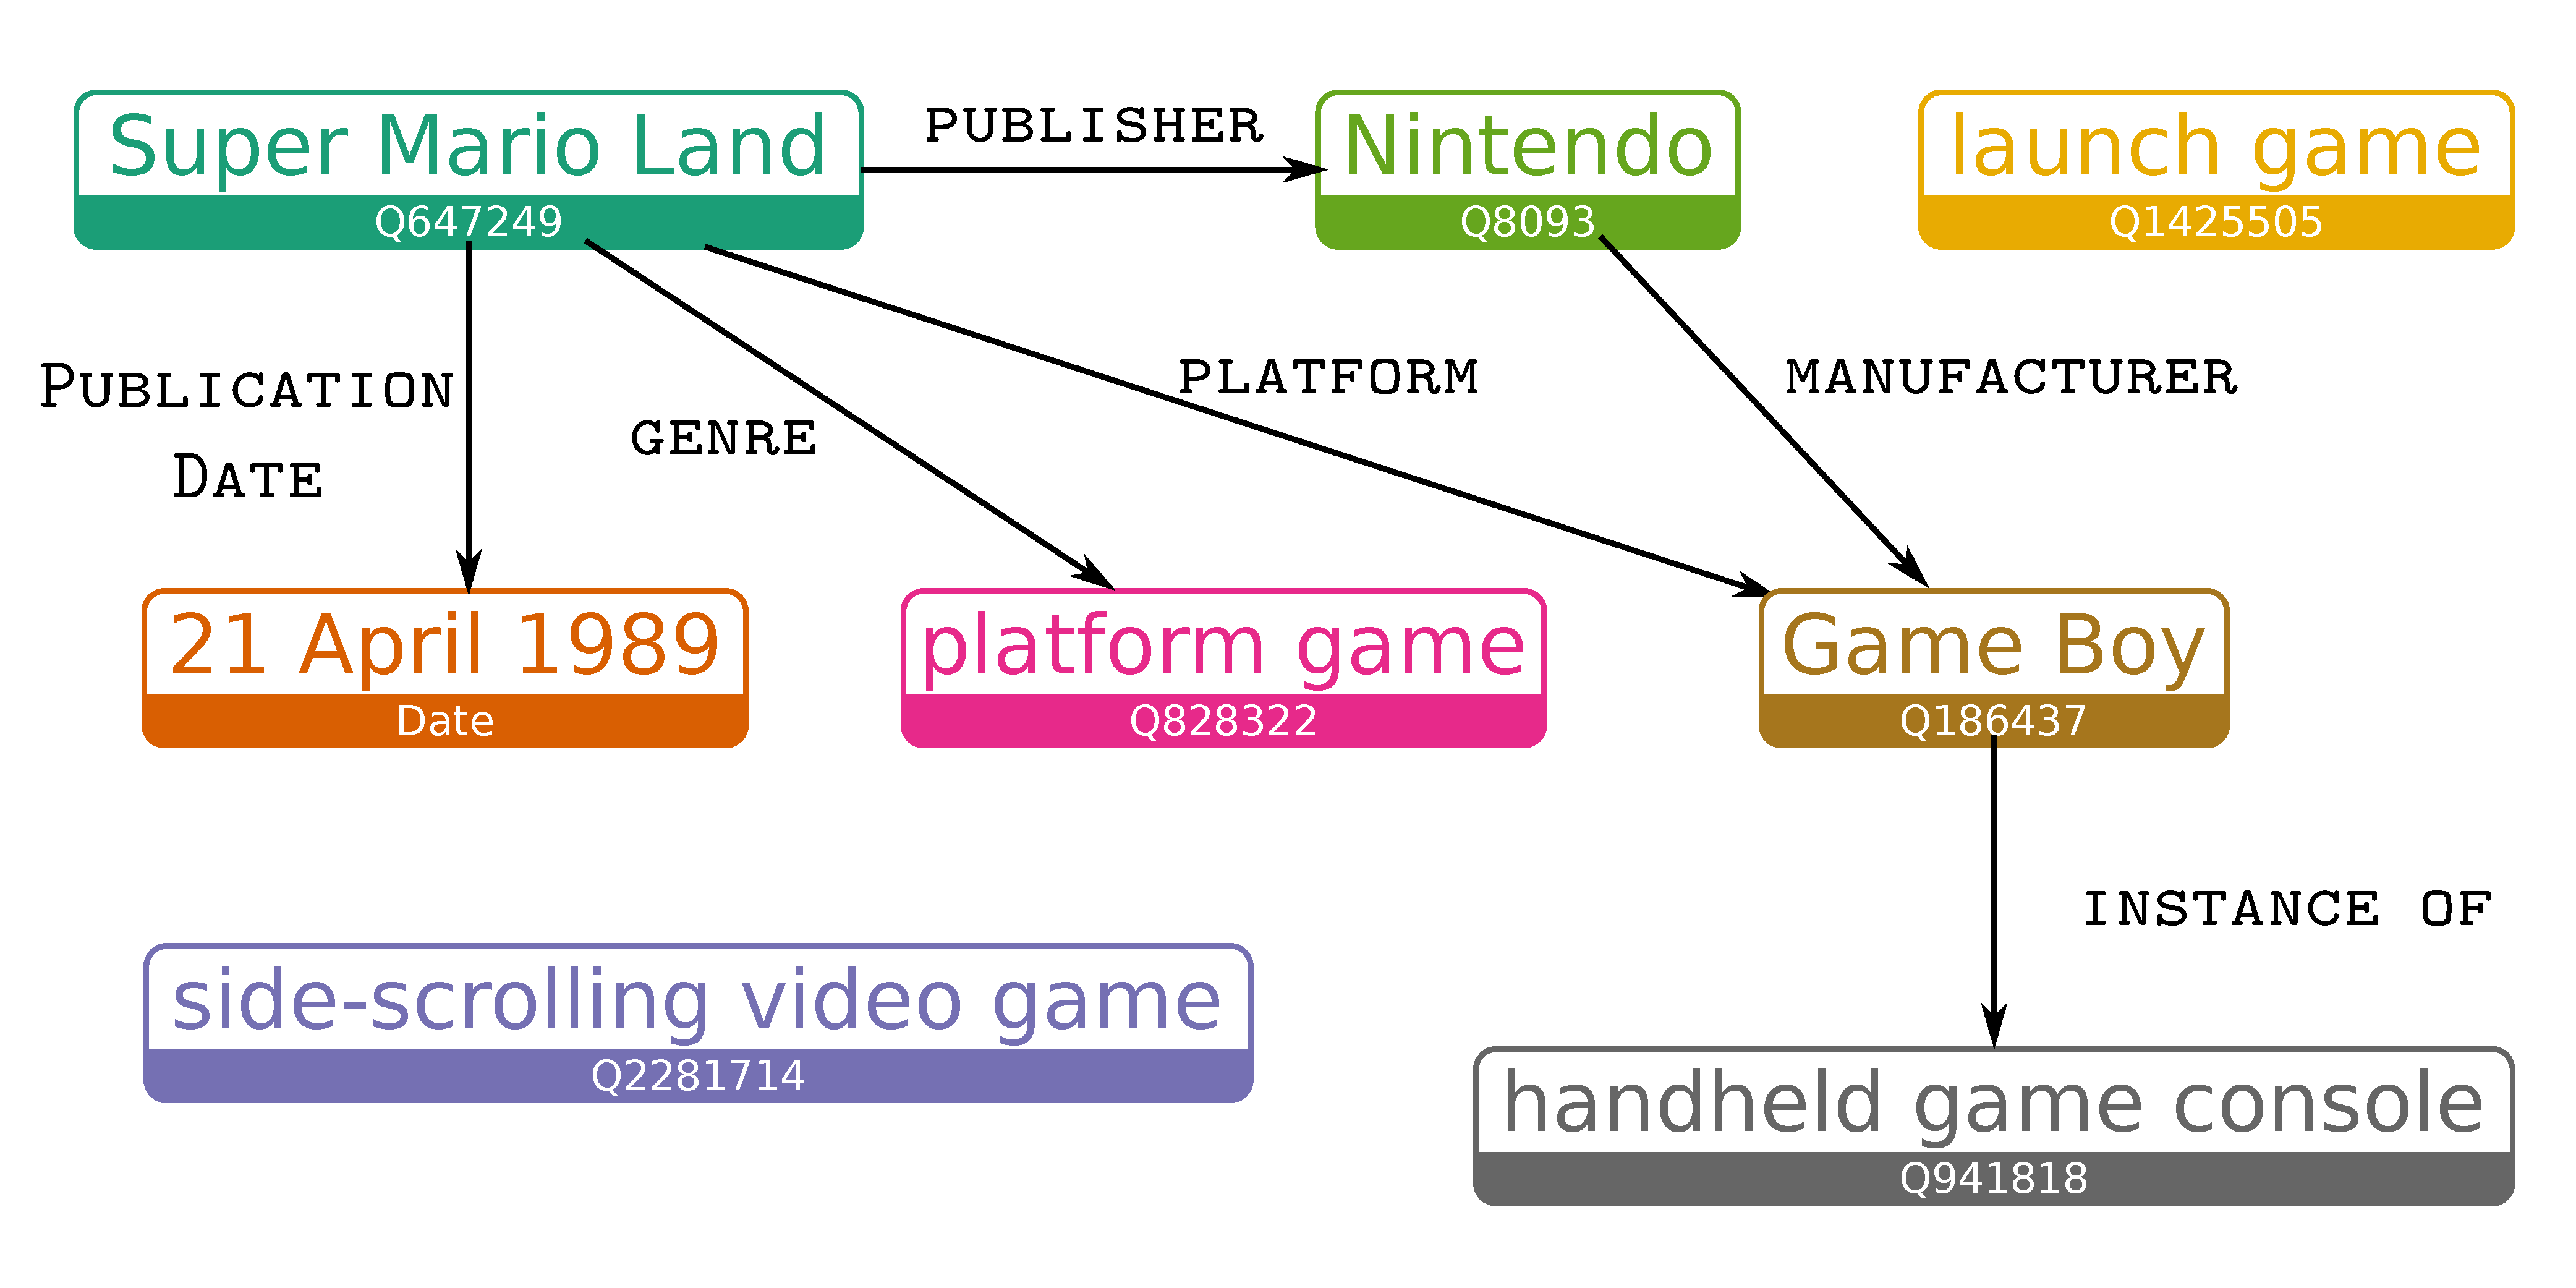
\includegraphics[width=0.8\linewidth]{figures/multimodality/mario_knowledge_graph.pdf}
% \caption{Local knowledge graph built during the inference of \textit{[Super Mario Land] is a [1989] [side-scrolling] [platform video game] developed and published by [Nintendo] as a [launch title] for their [Game Boy] [handheld game console]}. Figure adapted from \citet{logan2019barack}.}
% \label{fig:mario_knowledge_graph}
% \end{figure}

% There are three structures used: a static knowledge graph $\mathcal{KG}$ and a local graph $\mathcal{KG}_{<i}$ containing already encountered entities and their relations in the prefix.
% The model uses an LSTM unit, the hidden state of which is split into three components $[h_x; h_p; h_r]$ used for: (1) the token type decision, (2) parent entity prediction and (3) relation prediction. When the model makes a decision to predict an unrelated entity, it is sampled by a simple projection to the entity embedding space:
% $$\text{softmax}(v_e \cdot (h_p + h_r))$$

% The predicted entity $e$ is then added together with its immediate neighbours to the local graph:
% $$\mathcal{KG}_{<i+1} = \mathcal{KG}_{<i} \cup \{(e, r, x)|(e, r, x) \in \mathcal{KG}\}$$

% In case of a related entity, the model first predicts the parent, then the relation and finally the entity itself. When there are multiple entities in the local graph matching the restriction of the parent and the relation, it is sampled at random. The following set of equations describes the model behaviour in case of a new entity.
% \begin{align*}
% & \texttt{Encoder:} & p_p(e_p) = \text{ softmax}(v_p \cdot h_p)\\
% & & p_r(r)\hspace{0.18cm} = \text{ softmax}(v_r \cdot h_p) \\
% & & \hspace{1.1cm} \text{ constrained by } \exists e: (e_p, r, e) \in \mathcal{KG}_{<i}\\
% & \texttt{Retriever:} & p_e \underset{\text{\tiny sample}}{\sim} \{(e_p, r, e) | (e_p, r, e) \in \mathcal{KG}_{<i}\} \\
% & \texttt{Model:} & p_m = \text{renderer}(p_e) \\
% & \texttt{Update knowledge base:} & \mathcal{KG}_{<i+1} = \mathcal{KG}_{<i} \cup \{(e, r, x)|(e, r, x) \in \mathcal{KG}\}
% \end{align*}

% The main motivation for this approach is factual correctness in language modelling.
% Furthermore, it grants a higher degree of explainability and also allows for tighter manipulation and control of the data the model is working with as changing an entity in a relation has a direct impact on the produced output.

% The primary application of this model was factually-aware language modeling.
% As evaluation, the authors provided factual language modelling accuracy, i.e. \textit{Barack's wife is \_\_\_.} and computed the accuracy.
% In comparison to GPT-2$_\textsc{Small}$ \citep{radford2019language}, which obtained 15\% accuracy, the knowledge enhanced model achieved 39\%, showing that the controllable knowledge access improves the performance.

% \subsection{Dense Passage Retrieval}
% % I reused this from the Artefact Retrieval Paper -Vilém

% \mrinmaya{Can we talk about retrieval enhanced language modelling e.g. REALM instead? DPR is cool but a bit different and not exactly relevant to this class.}

% We focus on DPR \citep{karpukhin2020dense} which describes a prototypical question-answering system built with knowledge base access and dense document embeddings.

% DPR uses two BERT models to compute the document and question embeddings at the \texttt{[CLS]} token (768-dimensional). They are then fine-tuned so that the inner product (or $L^2$  distance or cosine similarity) of these two vectors is a good measure for document relevancy.
% The retrieved passages are reranked by a combination of the original similarity and the BM25 model \citep{robertson1995okapi}.
% For every retrieved passage, the probability of a span (up to fixed maximum length) being selected is computed as the product of two tokens (representation from another BERT model) being the start and end ones, respectively. 
% Reranking of the answers is done implicitly by choosing the span with the highest probability across all spans.
% The maximum similarity search is approximated to make it computationally feasible using FAISS \citep{johnson2019billion}.
% % 
% \begin{align*}
% & \texttt{Encoder:} & k = \textsc{Bert}_\text{query}(q)\\
% & \texttt{Knowledge base:} & \mathcal{B} = \{ \textsc{Bert}_\text{doc}(d) |d \in \mathcal{KB} \} \\
% & \texttt{Retriever:} & C = \arg \max^n_{d\in B} \text{sim}(q, d) \\
% & & C' = \text{Reranker}(C) \\
% & & \text{score given by: } \textsc{BM25}(q,d) + \lambda \cdot \text{sim}(q,d) \\
% & \texttt{Model:} & P_{\text{start},i}(s) = \text{softmax}(C'_i w_\text{start})_s \\
% & & P_{\text{end},i}(t) = \text{softmax}(C'_i w_\text{end})_t \\
% & & P_{\text{selection}}(i) = \text{softmax}(C' w_\text{selection})_i \\
% \end{align*}

% For every passage, $P_\text{selection}(i)$ is the score that this passage contains the answer and for every span $P_{\text{start},i}(s) \cdot P_{\text{end},i}(t)$ is the score of a single span ($s$ to $t$) in a passage.
% In this specific model, the aggregator simply passes on all the retrieved passages, though some models simply concatenate all passages and pass it to the model as single string input \citep{izacard2021leveraging}.

% Although useable in a language model, DPR was used primarily for question answering.
% On Natural Questions \citep{kwiatkowski2019natural}, it achieved the exact match score of 42 in contrast to BERT-based \citep{devlin-etal-2019-bert,lee2019latent} approach, which yielded the score of 27.
% \mrinmaya{If we keep this might want to include a bit more of results.}


% \subsection{KnowBERT}
% \TODO{remove}
% KnowBERT~\citep{DBLP:conf/emnlp/PetersNLSJSS19} is one typical knowledge-enhanced language model that injecting factual knowledge into \textit{hidden representations} of tokens. The idea is quite intuitive: if a language model can align mentions in the input text with entities in the knowledge base, we can say that factual knowledge is contained in this model. 
% %
% Note that in previous sections, we mentioned that in Transformers, text is first tokenized and vectorized as embeddings. Then, they are processed by Transformer modules. In KnowBERT, mentions are not aligned with entities before input into the model. Instead, they are both first vectorized, and then they are aligned in the format of hidden representations. 
% Next, we illustrate its idea with more details.

% \paragraph{Preparation (knowledge base and base language model).} 
% Knowledge bases contain rich factual knowledge. The knowledge in them is usually formatted as triples, i.e., (\texttt{subj}, \texttt{rel}, \texttt{obj}). \texttt{subj} and \texttt{obj} here are entities, which are usually associated with entity labels and descriptions. \texttt{rel} indicates the relationship between entities, with labels associated as well.
% In most cases, the knowledge is vectorized before usage. In KnowBERT, they compute entity embeddings from WordNet as the entity embeddings, where they claimed that relations, and synset definitions are encoded.

% As most knowledge-enhanced language models, KnowBERT is not trained from scratch. The \textbf{backbone pretrainded language model} is BERT, where we can regard the knowledge enhancement process as secondary pretraining or special finetuning of BERT. The architecture is roughly the same to BERT, with specially designed context mechanism.
% Next, we introduce the \textit{Knowledge Attention and Recontextualization} (as shown in Figure~\ref{fig:chp4-knowbert}) component with details.

% \begin{figure}
%     \centering
%     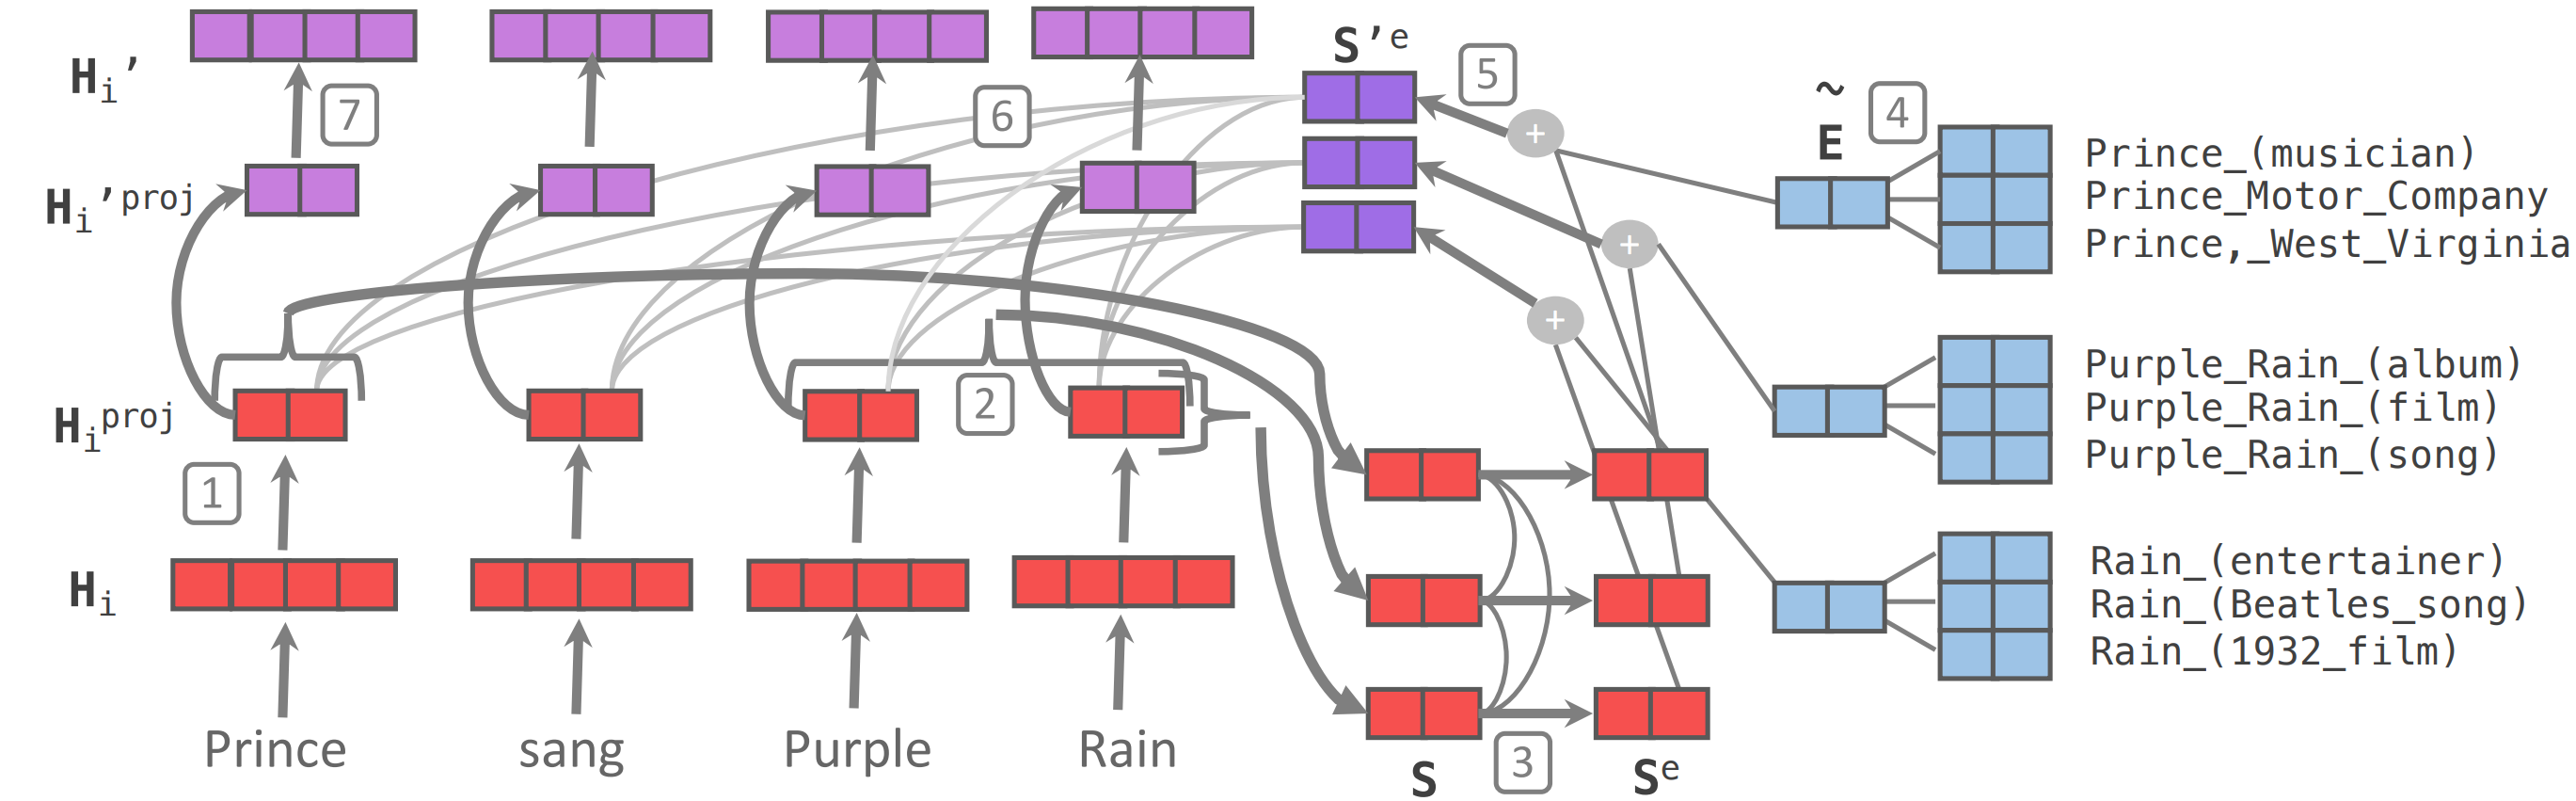
\includegraphics[width=\textwidth]{figures/knowbert.png}
%     \caption{The knowledge integration component of KnowBERT (i.e., Knowledge Attention and Recontextualization). BERT word piece representations $\texttt{\textbf{H}}_i$ are first projected to $\texttt{\textbf{H}}_i^\texttt{proj}$ (1), then pooled over candidate mentions spans (2) to compute $\texttt{\textbf{S}}$, and contextualized into $\texttt{\textbf{S}}^e$ using mention-span self-attention (3). An integrated entity linker computes weighted average entity embeddings $\widetilde{\texttt{\textbf{E}}}$ (4), which are used to enhance the span representations with knowledge from the knowledge base (5), computing $\texttt{\textbf{S}}^{'e}$. Finally, the BERT word piece representations are recontextualized with word-to-entity-span attention (6) and projected back to the BERT dimension (7) resulting in $\texttt{\textbf{H}}_i^{'}$.}
%     \label{fig:chp4-knowbert}
% \end{figure}

% \paragraph{(1) Mention-span representations} is calculated with below equation:
% \begin{equation}
%     \texttt{\textbf{H}}_i^\texttt{proj} = \texttt{\textbf{H}}_i \texttt{\textbf{W}}_1^\texttt{proj} + \texttt{\textbf{b}}_1^\texttt{proj}.
% \end{equation}
% The KAR starts with the knowledge base entity candidate selector that provides a list of candidate mentions which it uses to compute $C$ mention-span representations $\texttt{\textbf{s}}_m \in \mathbb{R}^{E}$. $\texttt{\textbf{H}}_i$ is first projected to the entity dimension with a linear projection, then, the KAR computes mention-span representations, one for each candidate mention, by pooling over all word pieces in a mention-span using the self-attentive span pooling. The mention-spans are stacked into a matrix $\texttt{\textbf{S}} \in \mathbb{R}^{C\times E}$.

% \paragraph{(2) Entity linker} functions as its name. Here, it is responsible for performing entity disambiguation for each potential mention from available candidates. It first runs mention-span self-attention to compute embedding as
% \begin{equation}
%     \texttt{\textbf{S}}^{e} = \text{TransformerBlock}(\texttt{\textbf{S}}).
% \end{equation}
% The span self-attention is identical to the typical transformer layer, exception that the attention mechanism here is \textbf{cross-attention}, which is between mention-span vectors instead of word piece vectors. This allows KnowBERT to incorporate global information into each linking decision, so that it can take advantage of entity-entity cooccurrence and resolve which of several overlapping candidate mentions should be linked.

% The objective function is based on the supervision signal of entity linking, which can be used to optimize parameters of the entity linker and other weight matrices.
% Specifically, $\texttt{\textbf{S}}^{e}$ is used to score each of the candidate entities while incorporating the candidate entity prior from the knowledge base. Each candidate span $m$ has an associated mention-span vector $\texttt{\textbf{s}}_m^{e} \in \texttt{\textbf{S}}^{e}$, $M_m$ candidate entities with embeddings $\texttt{\textbf{e}}_{mk}$ (from knowledge base), and prior probabilities $p_{mk}$. KnowBERT computes $M_m$ scores
% using the prior and dot product between the entity span vectors and entity embeddings as 
% \begin{equation}
%     \psi_{mk} = \text{MLP}(p_{mk}, \texttt{\textbf{s}}_m^{e}\cdot \texttt{\textbf{e}}_{mk}).
% \end{equation}
% And thus correspondingly, the loss function of entity linker can be written as
% \begin{equation}
%     \mathcal{L}_{\text{EntityLinker}} = - \sum_{m} \log{\left( \frac{\exp{\psi_{mg}}}{\sum_{k}{\exp{\psi_{mg}}}} \right)}
% \end{equation}

% \paragraph{(3-5) Knowledge enhanced entity-span representations.} 
% KnowBERT injects the knowledge base entity information into the mention-span representations computed from BERT vectors ($\texttt{\textbf{s}}_m^{e}$) to form entity span representations.
% The weighted entity embedding can be then written as 
% \begin{equation}
%     \widetilde{\texttt{\textbf{e}}}_m = \sum_{k} \psi_{mg} \texttt{\textbf{e}}_m.
% \end{equation}
% Then, the entity-span representations are updated with the weighted entity embeddings as
% \begin{equation}
%     \texttt{\textbf{s}}_m^{'e} = \texttt{\textbf{s}}_m^{e} +  \widetilde{\texttt{\textbf{e}}}_m,
% \end{equation}
% which can be packed into a matrix as $\texttt{\textbf{S}}^{'e} \in \mathbb{R}^{C\times E}$.

% \paragraph{(6-7) Recontextualization} happens after updating the entity span representations with the weighted entity vectors. KnowBERT uses them to recontextualize the word piece representations. This is accomplished using a modified transformer layer that substitutes the multi-headed self-attention with a multi-headed attention between the projected word piece representations and knowledge enhanced entity span vectors.
% As introduced before, we have 
% \begin{equation}
%     \texttt{\textbf{H}}_i^\texttt{'proj} = \text{MLP}(\text{MultiHeadAttn}(\texttt{\textbf{H}}_i^\texttt{proj}, \texttt{\textbf{S}}^{'e}, \texttt{\textbf{S}}^{'e})).
% \end{equation}
% Then, $\texttt{\textbf{H}}_i^\texttt{proj}$ is projected back to the BERT dimension with a linear transformation and a residual connection added as:
% \begin{equation}
%     \texttt{\textbf{H}}_i^\texttt{'} = \texttt{\textbf{H}}_i^\texttt{'proj} \texttt{\textbf{W}}_2^\texttt{proj} + \texttt{\textbf{b}}_2^\texttt{proj} + \texttt{\textbf{H}}_i.
% \end{equation}

% \paragraph{Training process.} To avoid catastrophic forgetting, KnowBERT cannot be trained only using the entity linking supervision signal, the pretraining objectives of BERT should also be considered. Thus, simply speaking, the knowledge enhancement objective is defined as:
% \begin{equation}
%     \mathcal{L}_{\text{KnowBERT}} = \mathcal{L}_{\text{BERT}} + \mathcal{L}_{\text{EntityLinker}}.
% \end{equation}
% Note that there are many engineering tricks of the KnowBERT design. These tricks are commonly used in many knowledge-enhanced language models. In our following sections, we will leave out these tricks for simplicity.

% \subsection{ERNIE [Optional]}
% ERNIE~\citep{zhang-etal-2019-ernie} was proposed prior to KnowBERT, which utilized part of the design mentioned above in the KnowBERT section. Therefore, to avoid repeating content, we briefly introduce the general method design of ERNIE, and mainly focus on the difference between ERNIE and KnowBERT.

% \begin{figure}
%     \centering
%     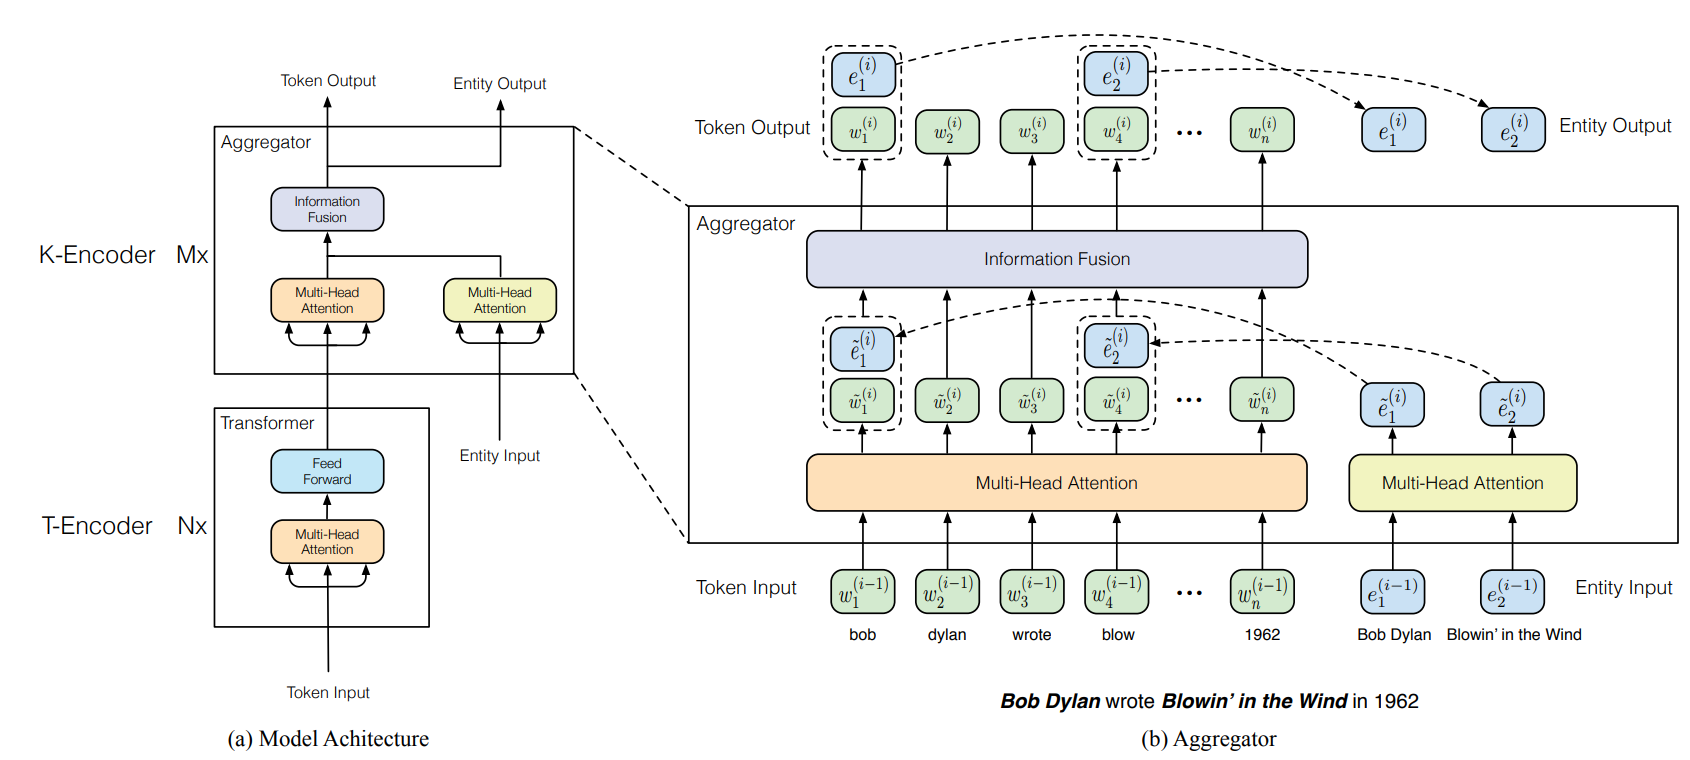
\includegraphics[width=\textwidth]{figures/ernie.png}
%     \caption{ The left part is the architecture of ERNIE. The right part is the aggregator for the mutual integration of the input of tokens and entities. Information fusion layer takes two kinds of input: one is the token embedding, and the other one is the concatenation of the token embedding and entity embedding. After information fusion, it outputs new token embeddings and entity embeddings for the next layer}
%     \label{fig:chp4-ernie}
% \end{figure}
% \paragraph{Architecture.} 
% The knowledge enhancement design of ERNIE can be found in Figure~\ref{fig:chp4-ernie}. 
% We can find that different from KnowBERT, the whole model architecture of ERNIE consists of two stacked modules: (1) the underlying textual encoder (T-Encoder) responsible to capture basic lexical and syntactic information from the input tokens, and (2) the upper knowledgeable encoder (K-Encoder) responsible to integrate extra token-oriented knowledge information into textual information from the underlying layer, so that we can represent heterogeneous information of tokens and entities into a united feature space.


% \paragraph{Objective.} 
% In order to inject knowledge into language representation by informative entities, ERNIE proposes a new pre-training task, which randomly masks some token-entity alignments and then requires the system to predict all corresponding entities based on aligned tokens. As the task is similar to training a denoising auto-encoder, it refers to this procedure as a denoising entity auto-encoder (dEA). 
% Considering that the size of entities is quite large for the softmax layer, ERNIE thus only requires the system to predict entities based on the given entity sequence instead of all entities in knowledge base. 
% Given the token sequence $\{w_1, ..., w_n\}$ and its corresponding entity
% sequence $\{e_1, ..., e_m\}$, the aligned entity distribution for the token $w_i$ is defined as follows,
% \begin{equation}
%     p(e_j| w_i) = \text{softmax}(\text{linear}(w_i^{o}) \cdot e_j). 
% \end{equation}
% The equation above will be used to compute the cross-entropy loss function for dEA.



% \paragraph{Performance.}
% After we know how KnowBERT and ERNIE inject knowledge, we show that they can perform good on knowledge-intensive tasks. 
% %
% Note that the knowledge enhancement can be regarded as the secondary pretraining. Thus, to compare the performance of BERT, ERNIE, and KnowBERT, similar to finetuning, we need first tune them on training data of the downstream task and then test them.
% %
% As aforementioned, the knowledge can be regarded as triples, which contains entities and relations. Thus, the most intuitive way to evaluate these knowledge-enhanced language models is to see if they perform good on predicting knowledge.


% \begin{table}[htbp]
% 	\smallskip
% 	\label{tab:knowbert_performance}
% 	\centering
%     \begin{tabular}{c|ccc|ccc}
%         \toprule
%         \multirow{2}*{\bf Model} &
%         \multicolumn{3}{c}{\bf Relation extraction} &
%         \multicolumn{3}{c}{\bf Entity typing} \\
%         % \cline{2-7}  
%         ~ & \bf Prec. & \bf Rec. & \bf $\bm{F_1}$-Micro & \bf Prec. & \bf Rec. & \bf $\bm{F_1}$-Micro  \\
%         \midrule  
%         \bf BERT & 67.2 & 64.8 & 66.0 & 76.4 & 71.0 & 73.6 \\
%         % \hline
%         \bf ERNIE & 70.0 &  66.1 & 68.0 & 78.4 & 72.9 & 75.6 \\
%         \bf KnowBERT & 71.6 &  71.4 & 71.5 & 78.6 & 73.7 & 76.1 \\
%         \bottomrule
%     \end{tabular}
% 	\caption{Performance of BERT, ERNIE, and KnowBERT on two knowledge-intensive tasks. \textbf{Prec.} = precision, \textbf{Rec.} = recall. Relation extraction by \citet{choi-etal-2018-ultra} and entity typing by \citet{zhang-etal-2017-position}.}
% \end{table} 

% We consider two typical knowledge-intensive downstream tasks for evaluation: relation extraction~\citep{choi-etal-2018-ultra} and entity typing~\citep{zhang-etal-2017-position}.
% Results can be found in \Cref{tab:knowbert_performance}. %The metric here is accuracy.
% \begin{itemize}
%     \item Relation extraction: Models are given a sentence with marked a subject and object, and asked to predict which of several different relations (or no relation) holds.
%     \item Entity typing: Given an entity mention and its context, entity typing requires systems to label the entity mention with its respective semantic types.
% \end{itemize}

